\documentclass[tikz,border=0pt,convert={density=1000,size=2000x1000,outext=.png}]{standalone}
\usepackage{tikz}

\usetikzlibrary{backgrounds,arrows,shapes,shapes.misc,shapes.arrows,chains,matrix,positioning,scopes,decorations.pathmorphing,shadows}

\tikzset{
    state/.style={
           rectangle,
           rounded corners,
           draw=black, very thick,
           minimum height=1em,
           inner sep=1pt,
           text centered,
           fill=gray
           },
}

\usepackage{amsmath,amssymb}

\usepackage{color}

\definecolor{light-gray}{gray}{0.9}
\begin{document}

\begin{footnotesize}

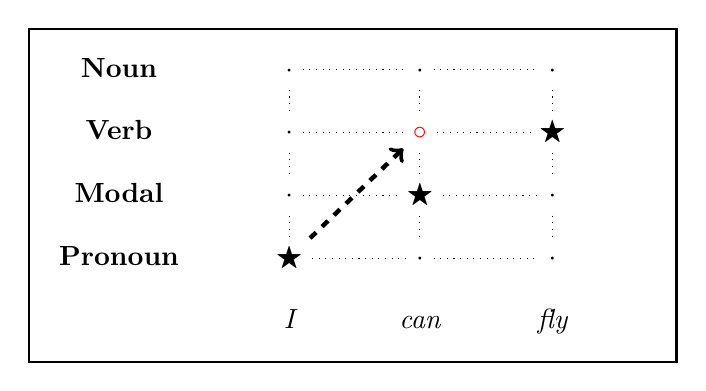
\begin{tikzpicture}[text height=1.5ex,text depth=.25ex,framed, background rectangle/.style={thick, draw=black}]
\matrix(m)[matrix of math nodes,column sep=1cm,row sep=0.3cm]{
    \textbf{Noun} &  \mathord{\cdot}   &\mathord{\cdot} &   \mathord{\cdot} &  \\
    \textbf{Verb} & \mathord{\cdot}  &\color{red}{\circ} &    \mathord{\bigstar} &    \\
    \textbf{Modal}  &\mathord{\cdot} & \mathord{\bigstar} &  \mathord{\cdot} &  \\
    \textbf{Pronoun} & \mathord{\bigstar}   &\mathord{\cdot} &   \mathord{\cdot} &  \\       
        & \textit{I} & \textit{can} &  \textit{fly} &  \\
};
\draw[dotted] 
(m-1-2)edge(m-2-2)
(m-2-2)edge(m-3-2)
(m-3-2)edge(m-4-2)
(m-1-3)edge(m-2-3)
(m-2-3)edge(m-3-3)
(m-3-3)edge(m-4-3)
(m-1-4)edge(m-2-4)
(m-2-4)edge(m-3-4)
(m-3-4)edge(m-4-4)
(m-1-2)edge(m-1-3)
(m-1-3)edge(m-1-4)
(m-2-2)edge(m-2-3)
(m-2-3)edge(m-2-4)
(m-3-2)edge(m-3-3)
(m-3-3)edge(m-3-4)
(m-4-2)edge(m-4-3)
(m-4-3)edge(m-4-4)
;

\draw[->,ultra thick, dashed]
(m-4-2)edge(m-2-3)
;

\end{tikzpicture}

	
\end{footnotesize}

\end{document}